\documentclass[a4paper,14pt]{extarticle}
\def\source{/home/osabio/tex/templates}
\input{\source/head.tex}
\yakovlev{306}{Магнитостатика}
% Стыдить лжеца, шутить над дураком
% И спорить с женщиной — всё то же,
% Что черпать воду решетом:
% От сих троих избавь нас, боже!..

% М. Ю. Лермонтов.
\usetikzlibrary{decorations.markings}
\usepackage[outline]{contour}
\contourlength{4pt}
\begin{document}

\begin{figure}[H]
    \centering
    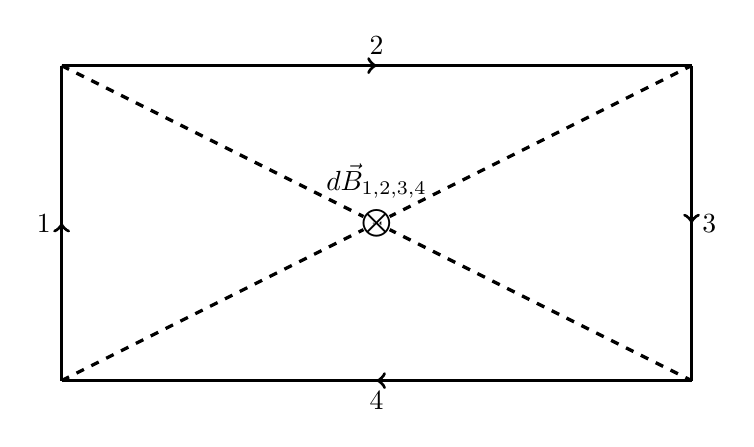
\begin{tikzpicture}
    % \begin{scope}[yshift=2cm]
    %     \lineann[2]{0}{-2}{$a$}
    % \end{scope}

    \begin{scope}[
        very thick,decoration={
        markings,
        mark=at position 0.5 with {\arrow{>}}}
        ] 
        \draw[postaction={decorate}] (0,0) coordinate (1)-- node[left] {1}(0,4);
        \draw[postaction={decorate}] (0,4) coordinate (2)-- node[above] {2}(8,4);
        \draw[postaction={decorate}] (8,4) coordinate (3)-- node[right] {3}(8,0);
        \draw[postaction={decorate}] (8,0) coordinate (4)-- node[below] {4}(0,0);

        \draw[dashed] (1) -- (3);
        \draw[dashed] (2) -- (4);
        % \draw[dashed] 
        %     (-4,4) node[above] {$O$}
        %     -- (0,0) node[anchor=west] {$A$}
        %     -- (4,-4) node[right] {$O'$};

        % \draw[dashed] 
        %     (4,4) node[above] {$B$}
        %     -- (-4,-4) node[right] {$B'$};            

        % \draw (135:{sqrt(2)}) node [] {\contour{white}{$\bigotimes$}}  node[above, yshift=0.5em] {$d\vec{B}_1$};
        \draw (4,2) node [] {\contour{white}{$\bigotimes$}} node[above, yshift=0.5em] {$d\vec{B}_{1,2,3,4}$};

        % \draw (45:{sqrt(2)}) node [] {\contour{white}{$\bigodot$}}  node[above, yshift=0.5em] {$d\vec{B}_1$};
        % \draw (45:2.5) node [] {\contour{white}{$\bigotimes$}} node[above, yshift=0.5em] {$d\vec{B}_2$};     

        % \draw (135+90:{sqrt(2)}) node [] {\contour{white}{$\bigotimes$}}  node[above, yshift=0.5em] {$d\vec{B}_1$};
        % \draw (135+90:2.5) node [] {\contour{white}{$\bigodot$}} node[above, yshift=0.5em] {$d\vec{B}_2$};

        % \draw (45-90:{sqrt(2)}) node [] {\contour{white}{$\bigodot$}}  node[above, yshift=0.5em] {$d\vec{B}_1$};
        % \draw (45-90:2.5) node [] {\contour{white}{$\bigodot$}} node[above, yshift=0.5em] {$d\vec{B}_2$};   

        % \draw (5,0) -- (14,0);          
        % \draw[] (9,-4) -- ++(0,8);          

    \end{scope}    
    \end{tikzpicture}
\end{figure}

Используем ранее выведенную формулу для произвольного отрезка проводника с током $B^p=\frac{\beta I}{a}[\sin\alpha_2-\sin\alpha_1]$.

Здесь $a$ --- расстояние от центра до стороны, равное половине другой стороны, а $\alpha_1=-\alpha_2\quad\Rightarrow\quad \sin\alpha_2-\sin\alpha_1=2\sin\alpha_2$: 


\begin{equation*}
    B_1=\frac{2\beta I}{a}2\frac{b}{\sqrt{a^2+b^2}}
\end{equation*}
\begin{equation*}
    B_2=\frac{2\beta I}{b}2\frac{a}{\sqrt{a^2+b^2}}
\end{equation*}
\begin{equation*}
    B_3=\frac{2\beta I}{b}2\frac{a}{\sqrt{a^2+b^2}}
\end{equation*}
\begin{equation*}
    B_4=\frac{2\beta I}{a}2\frac{b}{\sqrt{a^2+b^2}}
\end{equation*}

Тогда 

\begin{equation*}
    B=\sum B_i=4\beta I
    \left[
        \frac{b^2}{ab\sqrt{a^2+b^2}}+
        \frac{a^2}{ab\sqrt{a^2+b^2}}+
        \frac{a^2}{ab\sqrt{a^2+b^2}}+
        \frac{b^2}{ab\sqrt{a^2+b^2}}
    \right]
\end{equation*}

Откуда окончательно

\begin{equation*}
    B=8\beta I \frac{\sqrt{a^2+b^2}}{ab}
\end{equation*}


\end{document}